% ============================================================
% Customer Segmentation using RFM Analysis & K-Means Clustering
% Data Mining Project — Overleaf-compatible LaTeX Report
% ============================================================
\documentclass[12pt, a4paper]{article}

% ── Packages ─────────────────────────────────────────────────
\usepackage[utf8]{inputenc}
\usepackage[T1]{fontenc}
\usepackage{lmodern}
\usepackage[margin=2.5cm]{geometry}
\usepackage{graphicx}
\usepackage{booktabs}
\usepackage{array}
\usepackage{tabularx}
\usepackage{longtable}
\usepackage{amsmath, amssymb}
\usepackage{hyperref}
\usepackage{xcolor}
\usepackage{enumitem}
\usepackage{caption}
\usepackage{subcaption}
\usepackage{float}
\usepackage{listings}
\usepackage{fancyhdr}
\usepackage{setspace}
\usepackage[numbers]{natbib}

% ── Colours & Hyperlinks ────────────────────────────────────
\definecolor{linkblue}{HTML}{1a0dab}
\hypersetup{
    colorlinks = true,
    linkcolor  = linkblue,
    citecolor  = linkblue,
    urlcolor   = linkblue
}

% ── Headers / Footers ──────────────────────────────────────
\pagestyle{fancy}
\fancyhf{}
\fancyhead[L]{\footnotesize Customer Segmentation — RFM \& K-Means}
\fancyhead[R]{\footnotesize Data Mining Project}
\fancyfoot[C]{\thepage}
\renewcommand{\headrulewidth}{0.4pt}

% ── Code listing style ─────────────────────────────────────
\lstset{
    basicstyle   = \ttfamily\small,
    keywordstyle = \color{blue}\bfseries,
    commentstyle = \color{gray},
    stringstyle  = \color{red!70!black},
    breaklines   = true,
    frame        = single,
    xleftmargin  = 1em,
    framexleftmargin = 0.5em,
    numbers      = left,
    numberstyle  = \tiny\color{gray},
    language     = Python
}

% ── Spacing ─────────────────────────────────────────────────
\setstretch{1.15}

% ============================================================
\begin{document}

% ── Title Page ─────────────────────────────────────────────
\begin{titlepage}
    \centering
    \vspace*{2cm}
    
    {\Huge\bfseries Customer Segmentation using\\[0.4em]
     RFM Analysis \& K-Means Clustering\par}
    
    \vspace{1.5cm}
    {\Large Data Mining Project Report\par}
    
    \vspace{2cm}
    {\large
    % ── Replace with your name / team ──
    \textbf{Author Name}\\[0.3em]
    Department / University\\[0.3em]
    Course: Data Mining\\[0.3em]
    }
    
    \vspace{2cm}
    {\large \today\par}
    
    \vfill
    {\small An end-to-end customer segmentation study using RFM features\\
    and K-Means clustering on the Online Retail~II dataset.}
\end{titlepage}

% ── Table of Contents ──────────────────────────────────────
\newpage
\tableofcontents
\newpage

% ============================================================
\section{Introduction}\label{sec:intro}
% ============================================================

Picture a retailer sitting on two years of transaction logs and no clear way to tell which customers are worth nurturing and which ones have quietly disappeared. That was the starting problem for this project. Every customer in the dataset interacts with the store differently; some check in weekly, some dropped one order and never came back, some spend small amounts consistently while others make rare but large purchases. Grouping these people in a meaningful way, without any pre-existing labels, is the core analytical challenge we tried to answer.

The methodology follows \textbf{CRISP-DM}, a process model that moves through business understanding, data preparation, modelling, and evaluation in a deliberate sequence. What it prevented in practice was the temptation to jump into clustering before we'd properly interrogated the raw data. The main analytical tools are \textbf{RFM-based feature construction} paired with \textbf{K-Means Clustering}. Three per-customer summary statistics, how recently they bought, how many separate orders they placed, and how much they spent in total, turn a wide transaction table into a compact three-dimensional behavioural fingerprint that clustering algorithms can work with efficiently.

\subsection{Business Objective}

Once the pipeline ran end to end, the working dataset contained \textbf{5,001 customer profiles}, each described by a compact set of behavioural metrics. Splitting those profiles into groups isn't an end in itself; the value only materialises when each group maps to a concrete commercial decision. Several practical goals shaped how we defined ``useful'' segmentation:

\begin{itemize}[nosep]
    \item \textbf{Targeted marketing:} a campaign written for a specific customer type will always outperform a blanket message sent to everyone.
    \item \textbf{Customer retention:} customers who are slipping away give off detectable signals in their RFM numbers; catching that early changes what's still possible.
    \item \textbf{Resource allocation:} marketing budgets are finite, so spending more effort on high-potential segments and less on unreachable ones is just good economics.
    \item \textbf{Churn reduction:} acting on a fading relationship costs far less than running a recovery campaign after the customer has already left.
    \item \textbf{Revenue growth:} customers who are already engaged and spending are the most receptive to cross-sell and upgrade offers; segmentation identifies exactly who they are.
\end{itemize}

% ============================================================
\section{Dataset}\label{sec:dataset}
% ============================================================

The transaction records come from the \textbf{Online Retail~II} dataset, hosted on the UCI Machine Learning Repository~\cite{uci_retail}. It spans roughly two years of real purchase activity from a UK-based e-commerce store that sells gift-ware to a mix of direct consumers and wholesale buyers. Table~\ref{tab:dataset_overview} gives the key figures.

\begin{table}[H]
\centering
\caption{Dataset overview.}
\label{tab:dataset_overview}
\begin{tabular}{@{}ll@{}}
\toprule
\textbf{Property}   & \textbf{Value} \\
\midrule
Name                 & Online Retail II \\
Source               & UCI Machine Learning Repository \\
Sheets               & Year 2009--2010 (525,461 rows), Year 2010--2011 (541,910 rows) \\
Total Rows           & 1,067,371 transactions \\
Countries            & 43 \\
Date Range           & 2009-12-01 to 2011-12-09 \\
\bottomrule
\end{tabular}
\end{table}

\noindent The column names are mostly self-descriptive, but two of them carry non-obvious behaviour. Invoices beginning with \texttt{C} denote returns or cancellations, and \texttt{Customer ID} contains nulls wherever orders were placed without account registration. Both of those needed handling before any analysis could proceed. Table~\ref{tab:columns} captures the full schema.

\begin{table}[H]
\centering
\caption{Column schema of the Online Retail~II dataset.}
\label{tab:columns}
\begin{tabular}{@{}lll@{}}
\toprule
\textbf{Column} & \textbf{Type} & \textbf{Description} \\
\midrule
Invoice      & str      & Transaction ID (prefix \texttt{C} = cancellation) \\
StockCode    & str      & Product code \\
Description  & str      & Product name \\
Quantity     & int      & Units purchased (negative = return / cancellation) \\
InvoiceDate  & datetime & Date and time of transaction \\
Price        & float    & Unit price in GBP \\
Customer ID  & float    & Unique customer identifier (nullable) \\
Country      & str      & Customer country \\
\bottomrule
\end{tabular}
\end{table}

% ============================================================
\section{Data Preprocessing}\label{sec:preprocessing}
% ============================================================

Getting the data into a usable state took more time than any other single stage. Retail transaction exports are not clean by default; null identifiers, logged cancellations, negative stock quantities from returns, and duplicate rows all needed addressing before a single RFM value could be calculated. Each cleaning step is recorded in \texttt{src/preprocessing.py}:

\begin{enumerate}[nosep]
    \item \textbf{Remove null Customer IDs:} without an identifier, a row can't contribute to any per-customer aggregation; 243,007 such rows were dropped.
    \item \textbf{Remove cancelled transactions:} orders where the invoice starts with \texttt{C} record reversals, not purchases; 19,494 were excluded.
    \item \textbf{Remove non-positive Quantity:} values at or below zero indicate stock returns or data entry errors, not actual sales events.
    \item \textbf{Remove non-positive Price:} a unit price of zero or below doesn't reflect a real commercial transaction and was treated as erroneous.
    \item \textbf{Convert InvoiceDate} to \texttt{datetime64} so that date differences for the Recency calculation work correctly.
    \item \textbf{Remove duplicate rows:} 34,335 identical records were found and removed.
    \item \textbf{Create TotalPrice:} $\text{TotalPrice} = \text{Quantity} \times \text{Price}$ was derived here and used later when summing each customer's total spending.
\end{enumerate}

\noindent Table~\ref{tab:cleaning_summary} tracks the dataset size at each step.

\begin{table}[H]
\centering
\caption{Data cleaning summary.}
\label{tab:cleaning_summary}
\begin{tabular}{@{}lrr@{}}
\toprule
\textbf{Step} & \textbf{Rows Removed} & \textbf{Remaining} \\
\midrule
Initial dataset                      & ---       & 1,067,371 \\
Remove null Customer IDs             & 243,007   & 824,364   \\
Remove cancelled invoices (C-prefix) & 19,494    & 804,870   \\
Remove negative / zero Quantity      & varies    & $\sim$800,000 \\
Remove negative / zero Price         & varies    & $\sim$800,000 \\
Remove duplicate rows                & 34,335    & 779,425   \\
\midrule
\textbf{Clean dataset}              & ---       & \textbf{779,425} \\
\bottomrule
\end{tabular}
\end{table}

% ============================================================
\section{RFM Feature Engineering}\label{sec:rfm}
% ============================================================

With a clean dataset, collapsing the transaction table down to one row per customer was the next step. Each customer is characterised by three computed values, all anchored to a fixed reference point of \textbf{10 December 2011}, chosen as one day after the final recorded transaction. Table~\ref{tab:rfm_features} defines how each value is derived.

\begin{table}[H]
\centering
\caption{RFM feature definitions.}
\label{tab:rfm_features}
\begin{tabular}{@{}lll@{}}
\toprule
\textbf{Feature} & \textbf{Formula} & \textbf{Interpretation} \\
\midrule
Recency   & Days since last purchase  & How recently did the customer buy? \\
Frequency & Count of distinct invoices & How often do they buy? \\
Monetary  & $\sum (\text{Quantity} \times \text{Price})$ & How much do they spend in total? \\
\bottomrule
\end{tabular}
\end{table}

\subsection{Transformations}

Looking at the raw distributions of all three features, the spread is dramatically uneven. A handful of customers account for a large portion of total spend and order volume, which compresses most of the mass near the lower end of the scale. Feeding those raw values directly into K-Means would cause the algorithm to be dominated by outliers while most of the customer population collapses into a single undifferentiated group. Three sequential adjustments were made:

\begin{enumerate}[nosep]
    \item \textbf{Log transformation:} applying $\log(1+x)$ to each feature pulls the long tails inward and makes the distributions more symmetric. The $+1$ offset is included so that values of zero survive the transform without error.
    \item \textbf{IQR-based outlier removal:} after logging, residual extreme values were identified using a $1.5 \times \text{IQR}$ boundary per feature. Customers breaching any of the three boundaries were excluded; 877 were removed, leaving \textbf{5,001}.
    \item \textbf{Standardisation:} \texttt{StandardScaler} was applied last, shifting each feature to a mean of zero and scaling to unit variance. K-Means assigns points based on Euclidean distance, so features on different scales would otherwise distort every cluster boundary.
\end{enumerate}

\begin{figure}[H]
    \centering
    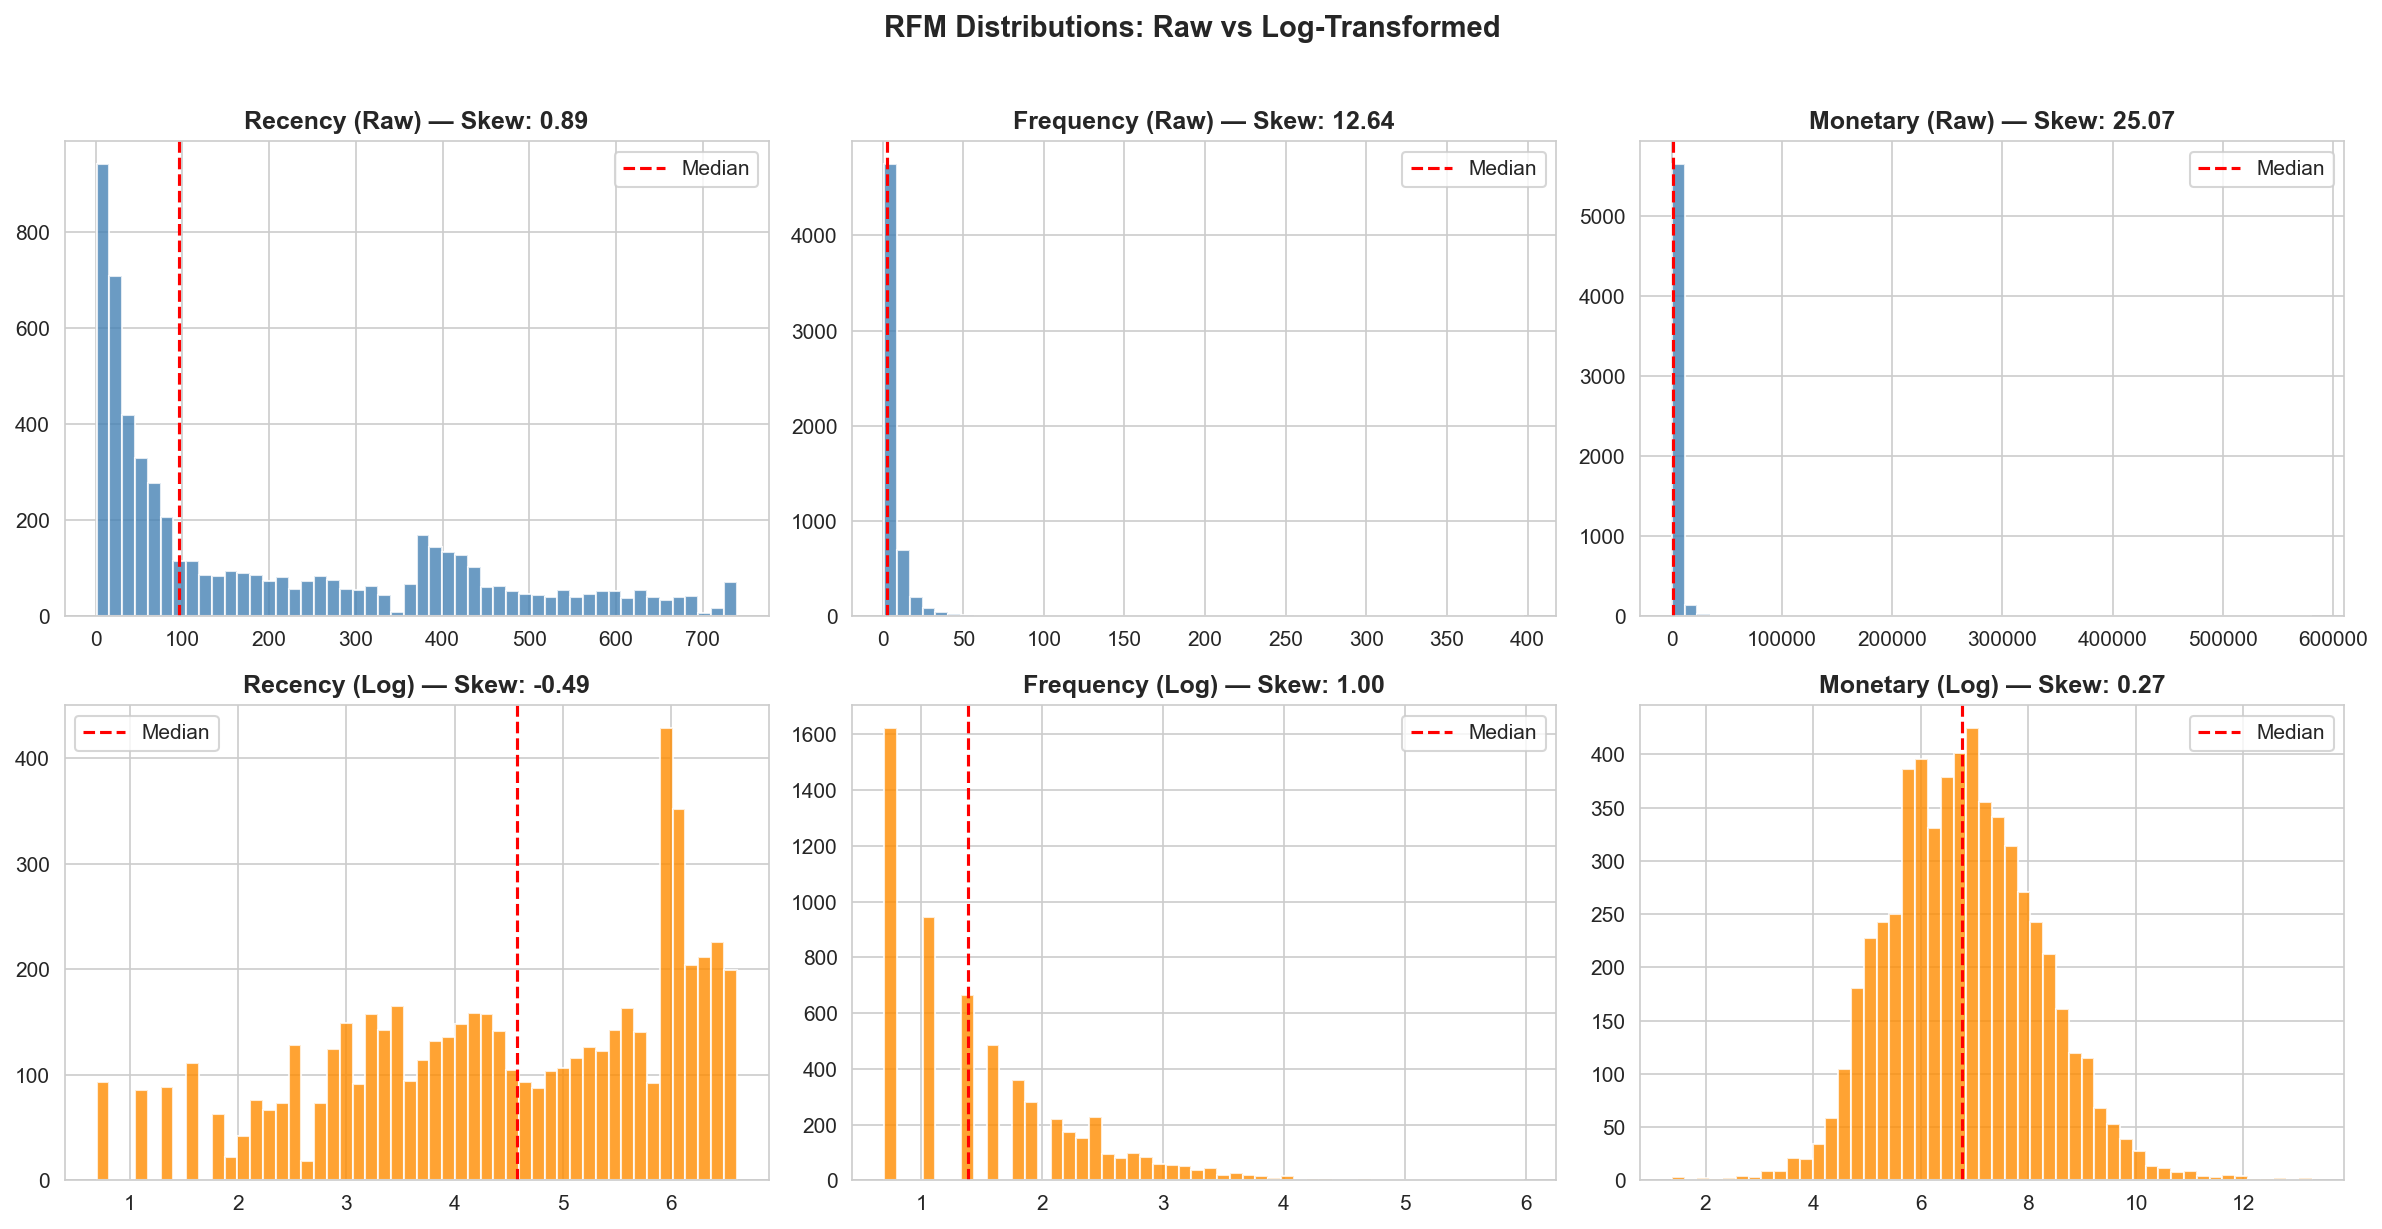
\includegraphics[width=\textwidth]{figures/rfm_raw_vs_log.png}
    \caption{Raw vs.\ log-transformed RFM distributions.}
    \label{fig:raw_vs_log}
\end{figure}

% ============================================================
\section{Exploratory Data Analysis}\label{sec:eda}
% ============================================================

Some time was spent examining the data visually before any models were built. The patterns that emerged shaped several decisions made later in the pipeline.

\subsection{Distribution Analysis}

Plotting raw Recency, Frequency, and Monetary as histograms shows distributions with a sharp peak near the low end and a very long right tail. After $\log(1+x)$ transformation, those same distributions take on a much more symmetric shape with a recognisable central tendency. Seeing both plots side by side made the case for the transformation far more convincingly than the skewness statistics alone.

\begin{figure}[H]
    \centering
    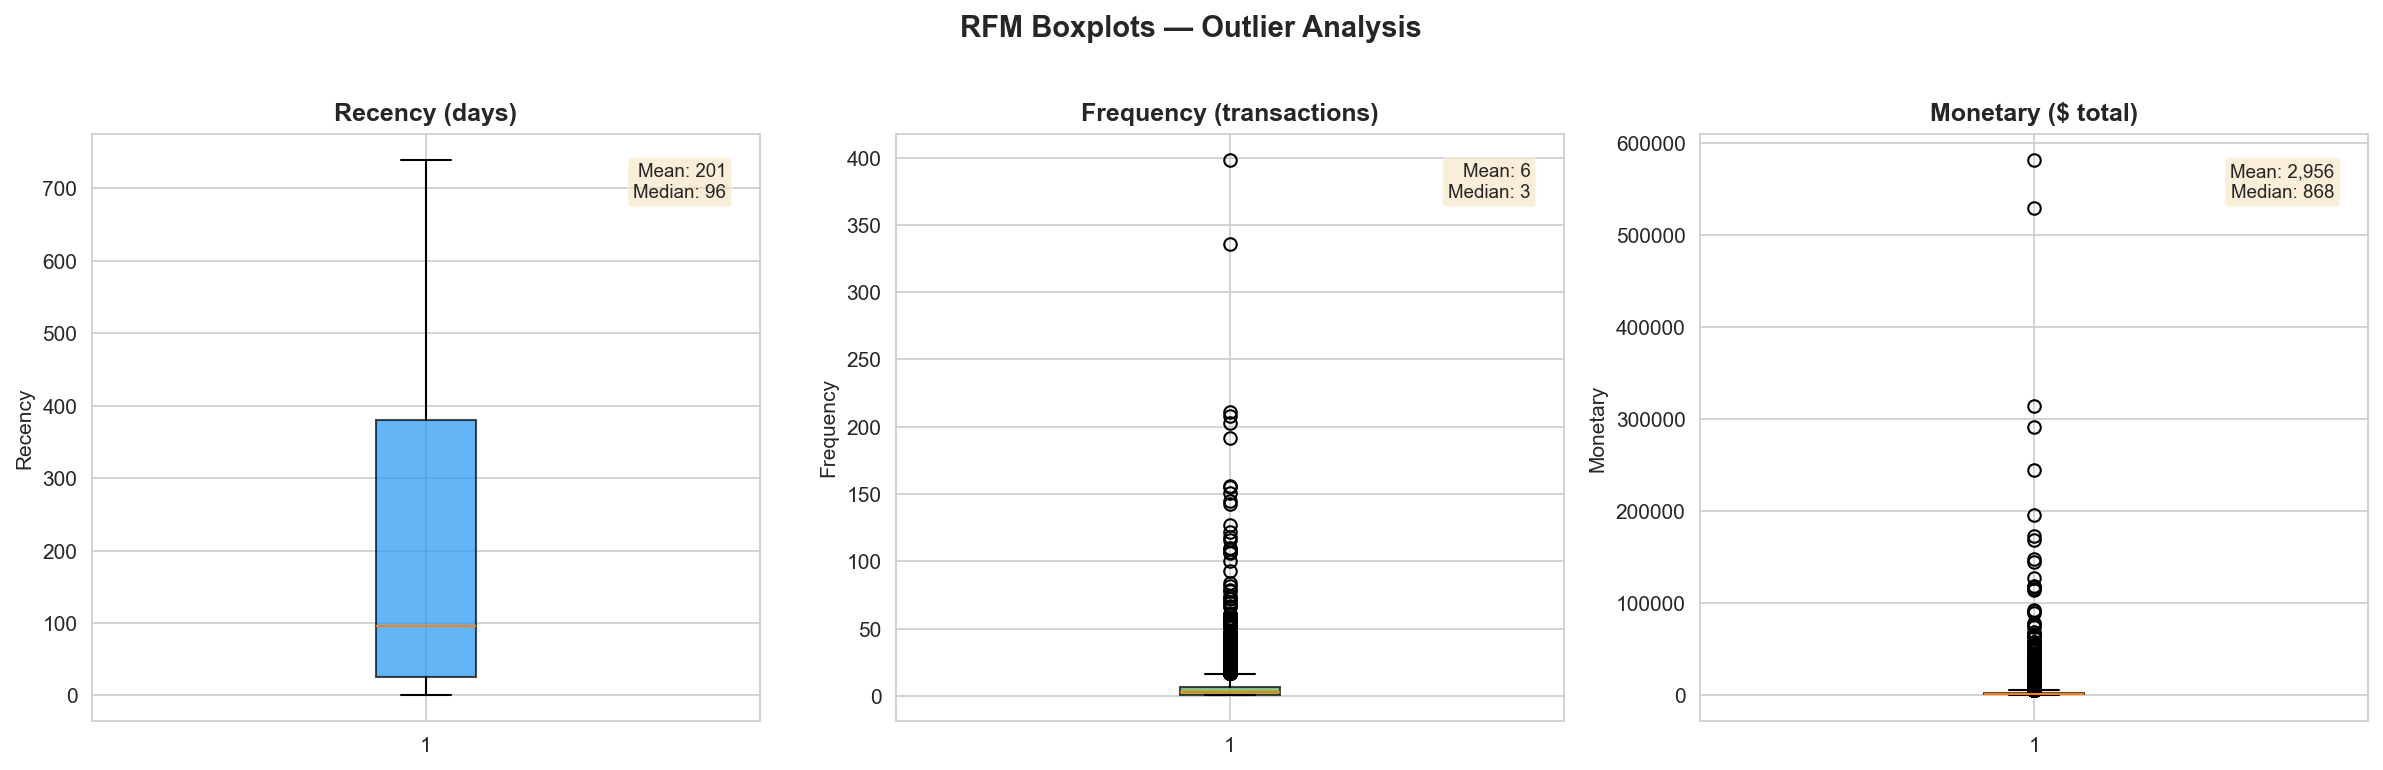
\includegraphics[width=0.85\textwidth]{figures/rfm_boxplots.png}
    \caption{RFM feature boxplots showing the spread and outlier distribution before removal.}
    \label{fig:rfm_boxplots}
\end{figure}

\subsection{Correlation Analysis}

Among the three features, Frequency and Monetary move together to a moderate degree, which follows logically from how they're defined. Customers who place more orders over the period will naturally accumulate higher total spend. Recency, by contrast, showed little linear association with either of the other two. That independence is actually useful; it suggests each feature is injecting different information into the clustering and none of the three is redundant.

\begin{figure}[H]
    \centering
    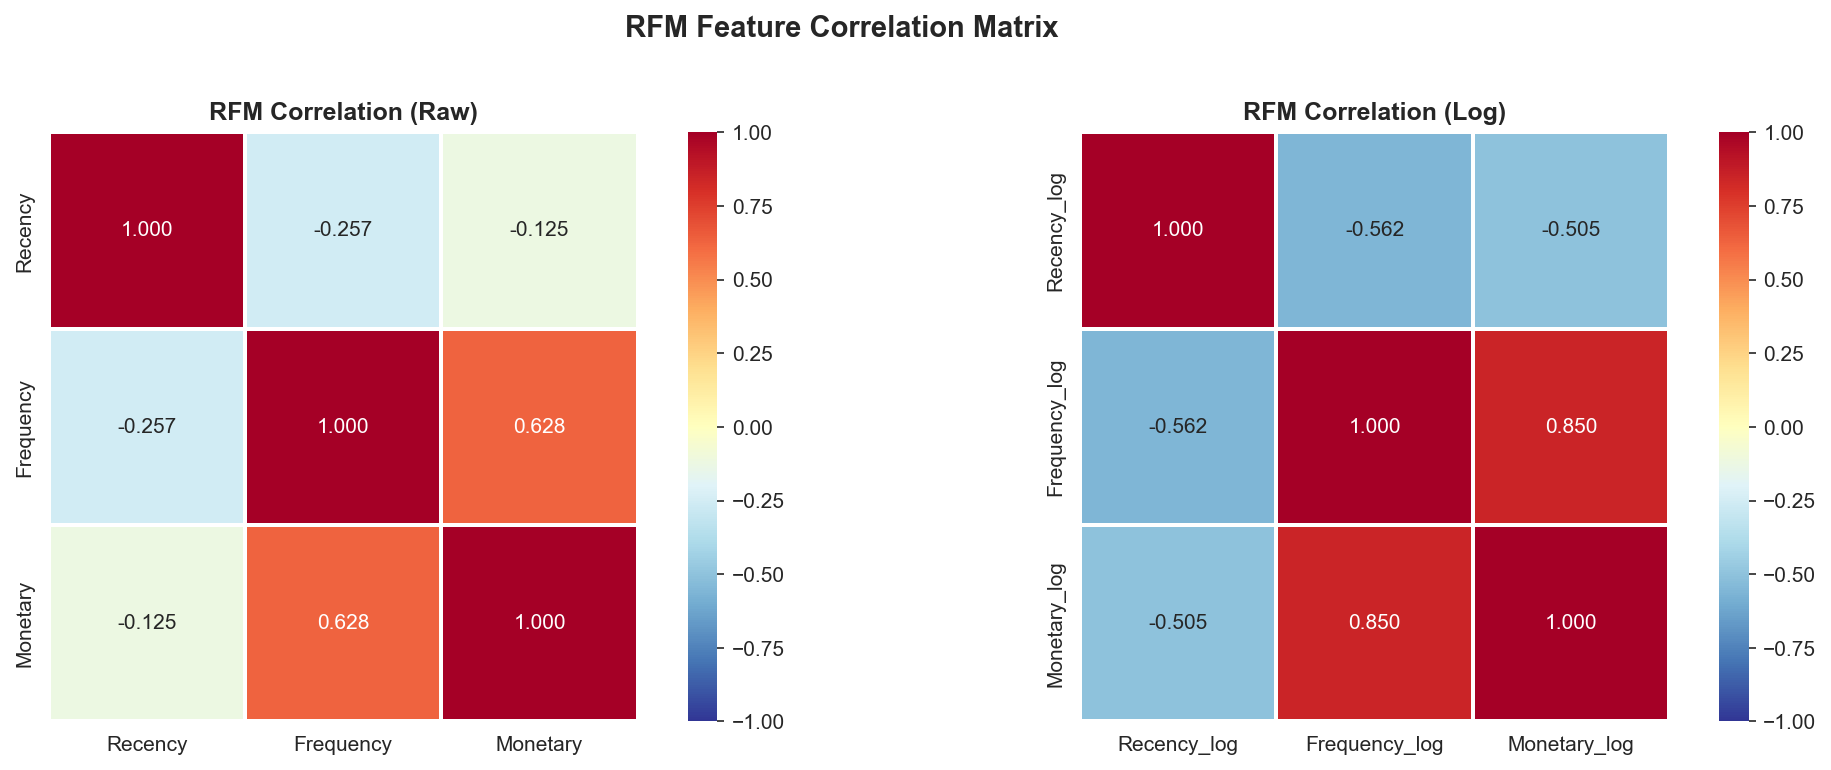
\includegraphics[width=0.65\textwidth]{figures/rfm_correlation.png}
    \caption{Pearson correlation heatmap of the three RFM features.}
    \label{fig:rfm_correlation}
\end{figure}

\subsection{Geographic Distribution}

The customer base is heavily concentrated in the \textbf{United Kingdom}, which dominates the count by a wide margin. Germany, France, and EIRE (Ireland) appear next, though at substantially lower volumes. The geographic spread is a useful contextual observation even if it didn't directly influence the segmentation approach.

\begin{figure}[H]
    \centering
    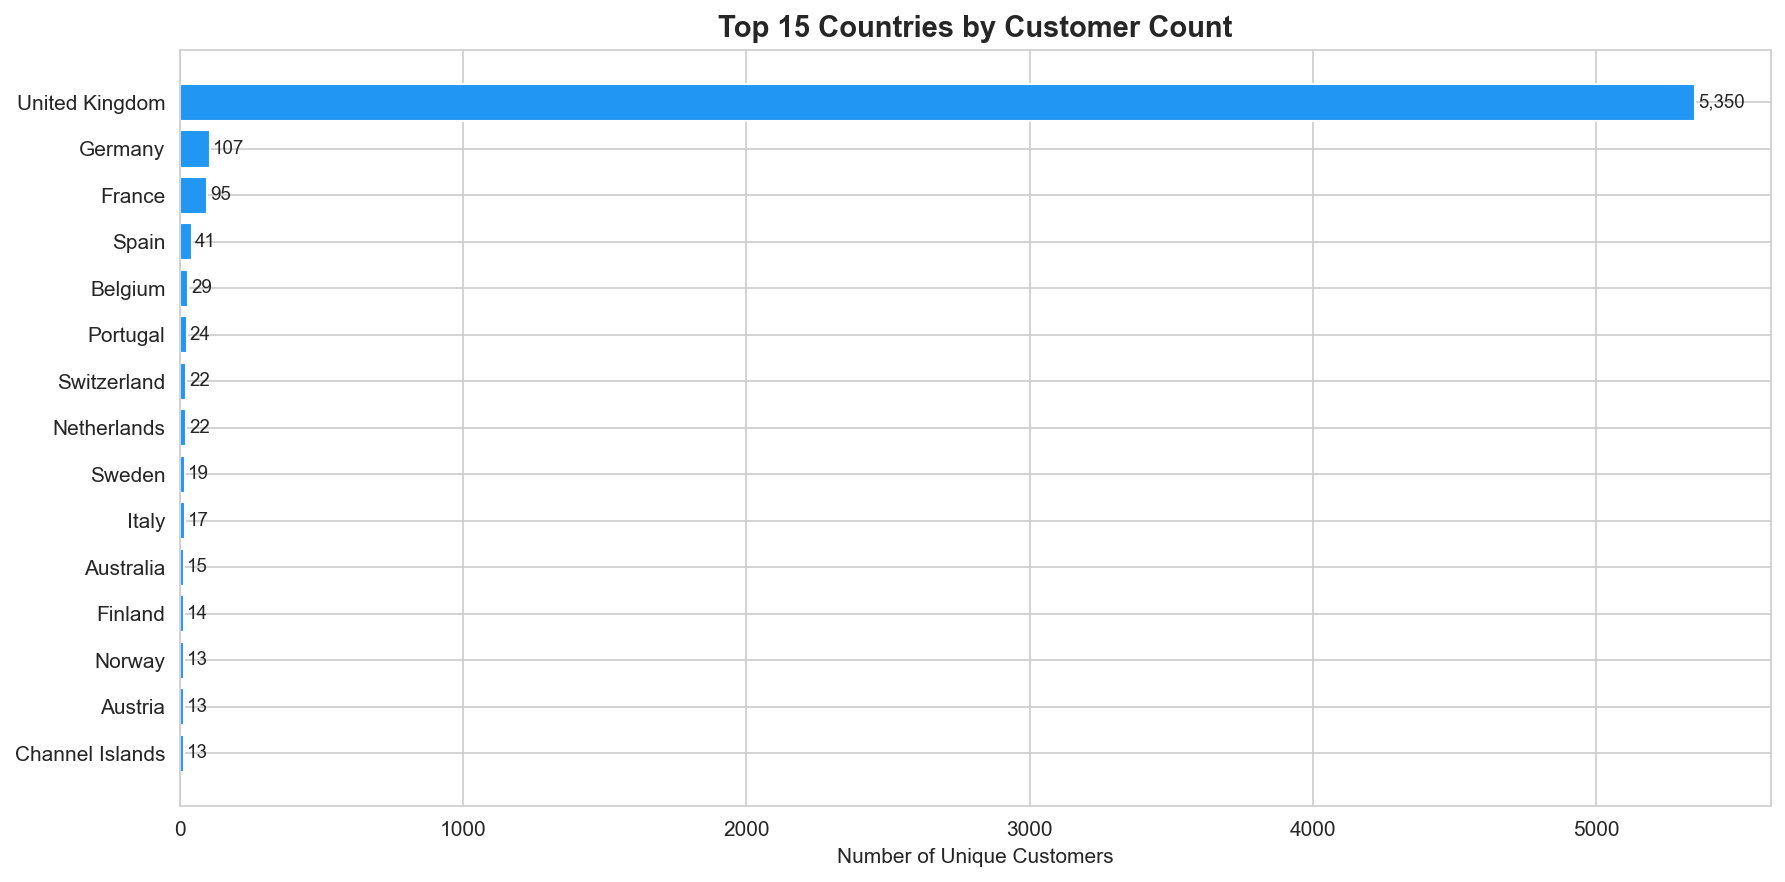
\includegraphics[width=0.85\textwidth]{figures/country_distribution.png}
    \caption{Top-15 countries by customer count.}
    \label{fig:country_distribution}
\end{figure}

% ============================================================
\section{Clustering Methodology}\label{sec:clustering}
% ============================================================

\subsection{Algorithm: K-Means}

K-Means suited this problem for a few practical reasons. Its computational overhead is low enough to support repeated runs across different configurations, the cluster assignments it produces are straightforward to explain to someone without a machine-learning background, and properly preprocessed features give it a good starting condition. The final parameter set is documented in Table~\ref{tab:kmeans_params}.

\begin{table}[H]
\centering
\caption{K-Means parameters.}
\label{tab:kmeans_params}
\begin{tabular}{@{}ll@{}}
\toprule
\textbf{Parameter} & \textbf{Value} \\
\midrule
\texttt{n\_clusters}   & 4 \\
\texttt{random\_state}  & 42 \\
\texttt{n\_init}        & 10 \\
\texttt{max\_iter}      & 300 \\
Scaler                  & StandardScaler \\
Features                & $\log(1+R)$, $\log(1+F)$, $\log(1+M)$ \\
\bottomrule
\end{tabular}
\end{table}

\subsection{Selecting the Number of Clusters}

Selecting $K$ is genuinely one of the harder decisions in a K-Means workflow because the data itself won't give you a single definitive answer. Two complementary diagnostics were used:

\begin{itemize}[nosep]
    \item \textbf{Elbow Method:} total within-cluster variance (inertia) is plotted against increasing values of $K$. The rate of improvement slows past a certain point, and the bend in that curve suggested $K=4$ as a sensible stopping point.
    \item \textbf{Silhouette Analysis:} for each data point, a score is computed that reflects how cohesive its own cluster is relative to the separation from its nearest neighbouring cluster. The result is a single number between $-1$ and $1$; values closer to $1$ indicate cleaner separation.
\end{itemize}

\noindent Table~\ref{tab:eval_metrics} records both metrics across the full range $K = 2$ to $10$.

\begin{table}[H]
\centering
\caption{K-Means evaluation metrics for $K=2\ldots10$.}
\label{tab:eval_metrics}
\begin{tabular}{@{}rrr@{}}
\toprule
\textbf{K} & \textbf{Inertia} & \textbf{Silhouette Score} \\
\midrule
2  & 7,625.05 & \textbf{0.4149} \\
3  & 5,883.70 & 0.3219 \\
\textbf{4}  & \textbf{4,404.41} & \textbf{0.3624} \\
5  & 3,763.18 & 0.3105 \\
6  & 3,272.71 & 0.3218 \\
7  & 2,912.64 & 0.2925 \\
8  & 2,653.04 & 0.2927 \\
9  & 2,456.93 & 0.2799 \\
10 & 2,287.89 & 0.2825 \\
\bottomrule
\end{tabular}
\end{table}

\noindent $K=2$ produces the strongest silhouette score at 0.4149, but the resulting partition splits customers into little more than two broad camps with limited commercial specificity. \textbf{$K=4$} was selected instead; its silhouette of \textbf{0.3624} is slightly lower, but the four clusters it produces each carry a recognisable behavioural signature that maps directly onto actionable business categories.

\subsection{Hierarchical Clustering Comparison}

As a cross-check, Agglomerative Clustering using Ward linkage was run at $K=4$. Ward linkage merges clusters by minimising the increase in total within-cluster variance at each step, which tends to produce compact, evenly sized groups. The dendrogram output showed four branches that aligned well with the K-Means boundaries, giving some confidence that the four-cluster structure isn't an artefact of the algorithm choice.

\begin{figure}[H]
    \centering
    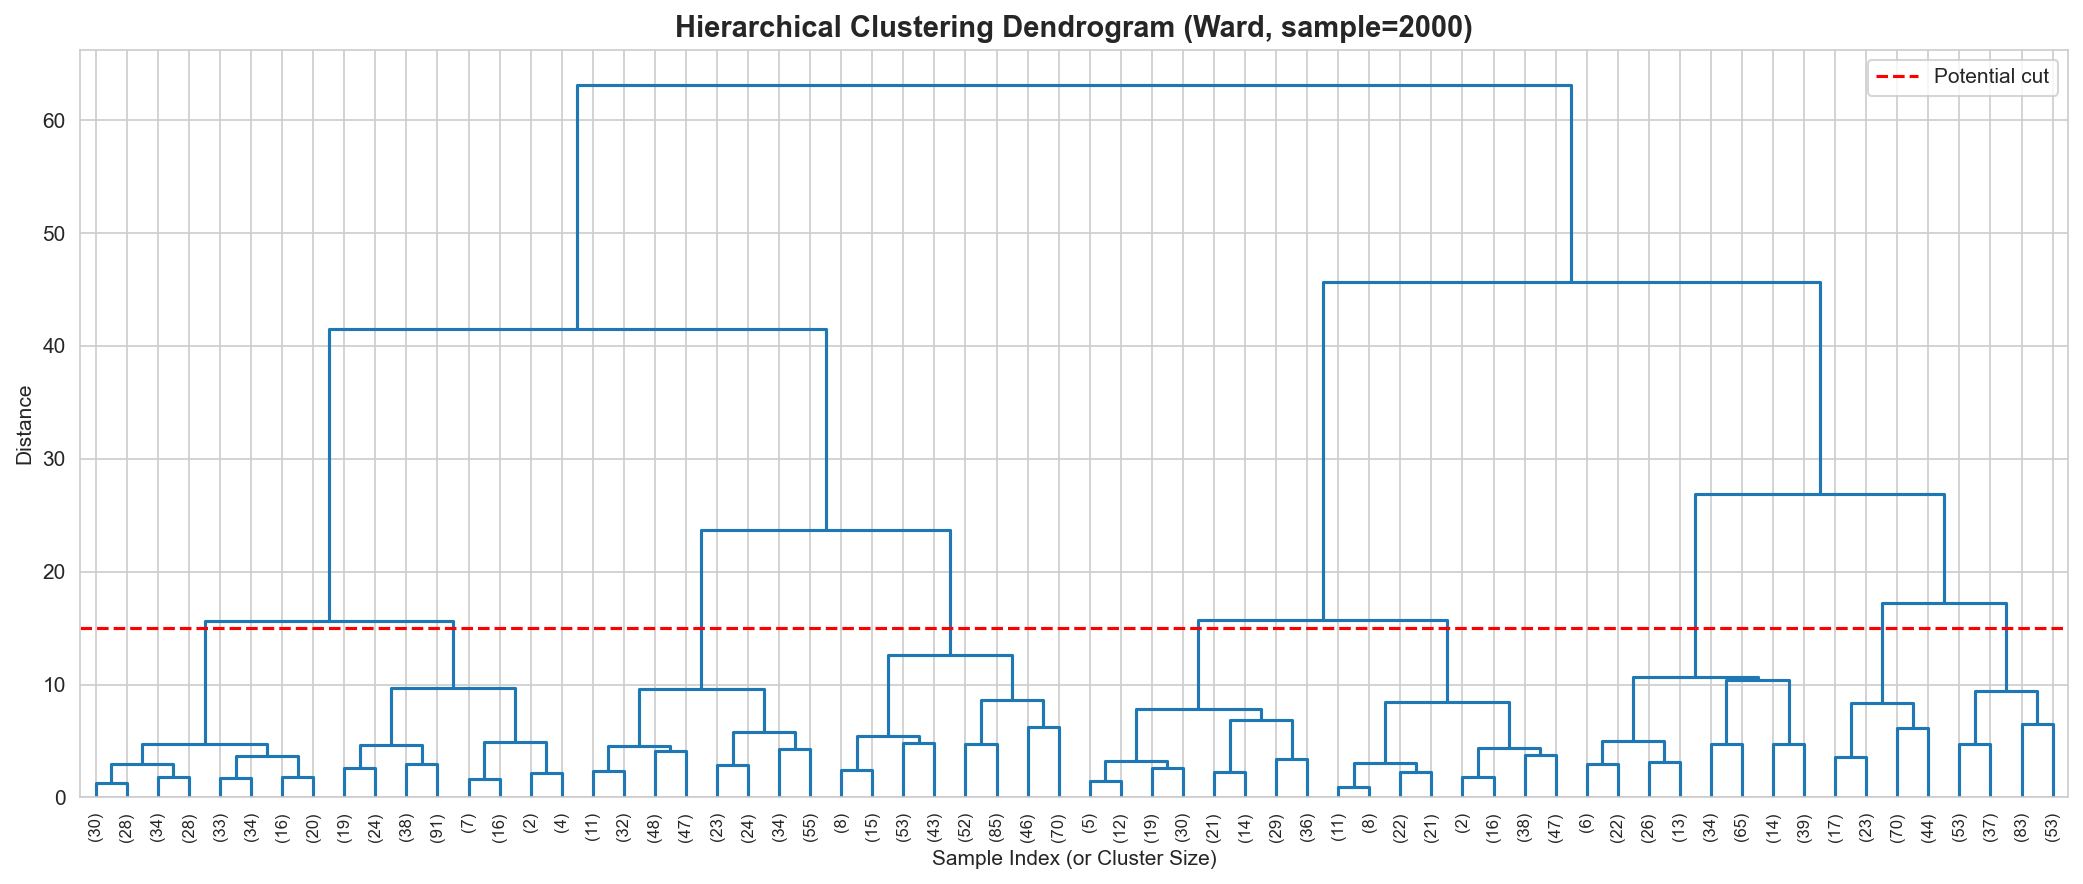
\includegraphics[width=0.85\textwidth]{figures/dendrogram.png}
    \caption{Hierarchical clustering dendrogram with Ward linkage.}
    \label{fig:dendrogram}
\end{figure}

% ============================================================
\section{Experimentation}\label{sec:experiments}
% ============================================================

To avoid over-fitting the pipeline to a single configuration, a structured comparison was run. Three feature scaling strategies were tested (StandardScaler, MinMaxScaler, and RobustScaler), each paired with $K \in \{3, 4, 5\}$ and run both before and after IQR outlier removal. The twelve resulting configurations are ranked by silhouette score in Table~\ref{tab:experiments}.

\begin{table}[H]
\centering
\caption{Experimentation results — scaler, outlier handling, and $K$.}
\label{tab:experiments}
\begin{tabular}{@{}llrrr@{}}
\toprule
\textbf{Scaler} & \textbf{Outlier Handling} & \textbf{K} & \textbf{Silhouette} & \textbf{Customers} \\
\midrule
MinMaxScaler    & IQR Removed   & 4 & \textbf{0.3944} & 5,001 \\
MinMaxScaler    & IQR Removed   & 3 & 0.3826          & 5,001 \\
StandardScaler  & With Outliers & 4 & 0.3650          & 5,878 \\
\textbf{StandardScaler} & \textbf{IQR Removed} & \textbf{4} & \textbf{0.3624} & \textbf{5,001} \\
RobustScaler    & IQR Removed   & 4 & 0.3603          & 5,001 \\
StandardScaler  & With Outliers & 3 & 0.3477          & 5,878 \\
MinMaxScaler    & IQR Removed   & 5 & 0.3462          & 5,001 \\
StandardScaler  & With Outliers & 5 & 0.3425          & 5,878 \\
RobustScaler    & IQR Removed   & 3 & 0.3277          & 5,001 \\
StandardScaler  & IQR Removed   & 3 & 0.3219          & 5,001 \\
RobustScaler    & IQR Removed   & 5 & 0.3171          & 5,001 \\
StandardScaler  & IQR Removed   & 5 & 0.3105          & 5,001 \\
\bottomrule
\end{tabular}
\end{table}

\noindent The top silhouette score (0.3944) belongs to MinMaxScaler combined with IQR removal at $K=4$. StandardScaler with the same outlier treatment scored 0.3624. The decision to use StandardScaler despite the lower score comes down to coherence: the log transformation applied earlier is a variance-stabilising step, and StandardScaler is the natural scaling companion to that; using MinMaxScaler would have re-introduced sensitivity to the boundary values that log transformation was intended to soften.

% ============================================================
\section{Results \& Cluster Profiles}\label{sec:results}
% ============================================================

Labelling clusters required a method that could operate without subjective intervention. A \textbf{rank-based composite scoring} system was used: each cluster receives a rank from 1 to 4 on each of the three RFM dimensions independently (Recency ranked lowest-value-first since a shorter gap is preferable; Frequency and Monetary ranked highest-value-first). Summing those three ranks gives a composite score, and the resulting ordering maps cleanly onto four recognisable customer archetypes. Table~\ref{tab:rfm_clusters} presents the complete picture.

\begin{table}[H]
\centering
\caption{Final cluster profiles with business labels.}
\label{tab:rfm_clusters}
\begin{tabular}{@{}clrrrrr@{}}
\toprule
\textbf{Cluster} & \textbf{Business Label} & \textbf{Count} & \textbf{\%} & \textbf{Avg R} & \textbf{Avg F} & \textbf{Avg M (\pounds)} \\
\midrule
0 & Hibernating / Lost       & 1,571 & 31.4 & 415 & 1.2  & 247   \\
1 & Loyal / Regular          & 982   & 19.6 & 35  & 2.2  & 613   \\
2 & Champions / High-Value   & 1,138 & 22.8 & 45  & 7.7  & 2,180 \\
3 & At-Risk / Declining      & 1,310 & 26.2 & 301 & 3.5  & 1,151 \\
\bottomrule
\end{tabular}
\end{table}

\subsection{Cluster Interpretation}

\paragraph{Cluster 2, Champions / High-Value Loyal (22.8\%)}
The numbers here are striking on every axis. Average recency of 45 days means these customers were purchasing very recently. Average transaction count of 7.7 is high by any standard in this dataset. Average spend of \pounds2,180 places them comfortably above every other group. Despite being just over a fifth of the total customer base, this cluster almost certainly accounts for a much larger proportion of revenue.

\paragraph{Cluster 1, Loyal / Regular Customers (19.6\%)}
Recency of 35 days puts this group among the most recently active. Frequency (2.2) and monetary (\pounds613) are more modest but still positive. These customers are in a good position; they haven't gone anywhere, and there's a reasonable path to increasing their value with the right kind of interaction.

\paragraph{Cluster 3, At-Risk / Declining Customers (26.2\%)}
What makes this cluster two is the contrast between their historical engagement and their current absence. Frequency at 3.5 and spend at \pounds1,151 suggest they were once reasonably active customers. But an average of 301 days without a purchase puts them firmly in the at-risk category. The gap between who they were and what the recency figure now shows is the signal worth acting on.

\paragraph{Cluster 0, Hibernating / Lost Customers (31.4\%)}
This is the largest group and the most difficult to recover. At 415 days average since last purchase, with an average of only 1.2 orders ever placed and total spend of \pounds247, many customers here likely made a single purchase and moved on. A re-engagement attempt is worth running, but the conversion rate is expected to be low.

% ============================================================
\section{Visualisations}\label{sec:visualisations}
% ============================================================

A range of plots was produced at different stages of the analysis. Some directly influenced modelling decisions; others served mainly as verification that earlier steps had worked as intended. Table~\ref{tab:visualisations} catalogues the full set.

\begin{table}[H]
\centering
\caption{Visualisation outputs generated by the pipeline.}
\label{tab:visualisations}
\small
\begin{tabular}{@{}ll@{}}
\toprule
\textbf{File} & \textbf{Description} \\
\midrule
\texttt{rfm\_raw\_vs\_log.png}          & Raw vs.\ log-transformed RFM histograms \\
\texttt{rfm\_correlation.png}           & Pearson correlation heatmap \\
\texttt{country\_distribution.png}      & Top-15 countries by customer count \\
\texttt{rfm\_boxplots.png}              & RFM feature boxplots (outlier view) \\
\texttt{elbow\_silhouette.png}          & Elbow + silhouette curves ($K=2\ldots10$) \\
\texttt{silhouette\_diagram.png}        & Per-sample silhouette plot for $K=4$ \\
\texttt{dendrogram.png}                 & Hierarchical dendrogram (Ward linkage) \\
\texttt{clusters\_pca.png}              & 2D PCA scatter by cluster \\
\texttt{clusters\_tsne.png}             & 2D t-SNE scatter by cluster \\
\texttt{cluster\_comparison\_bars.png}  & Mean R/F/M bar chart per cluster \\
\texttt{cluster\_radar.png}             & Radar chart of normalised RFM profiles \\
\texttt{cluster\_boxplots.png}          & RFM boxplots split by cluster \\
\texttt{cluster\_pie.png}               & Customer distribution pie chart \\
\bottomrule
\end{tabular}
\end{table}

\begin{figure}[H]
    \centering
    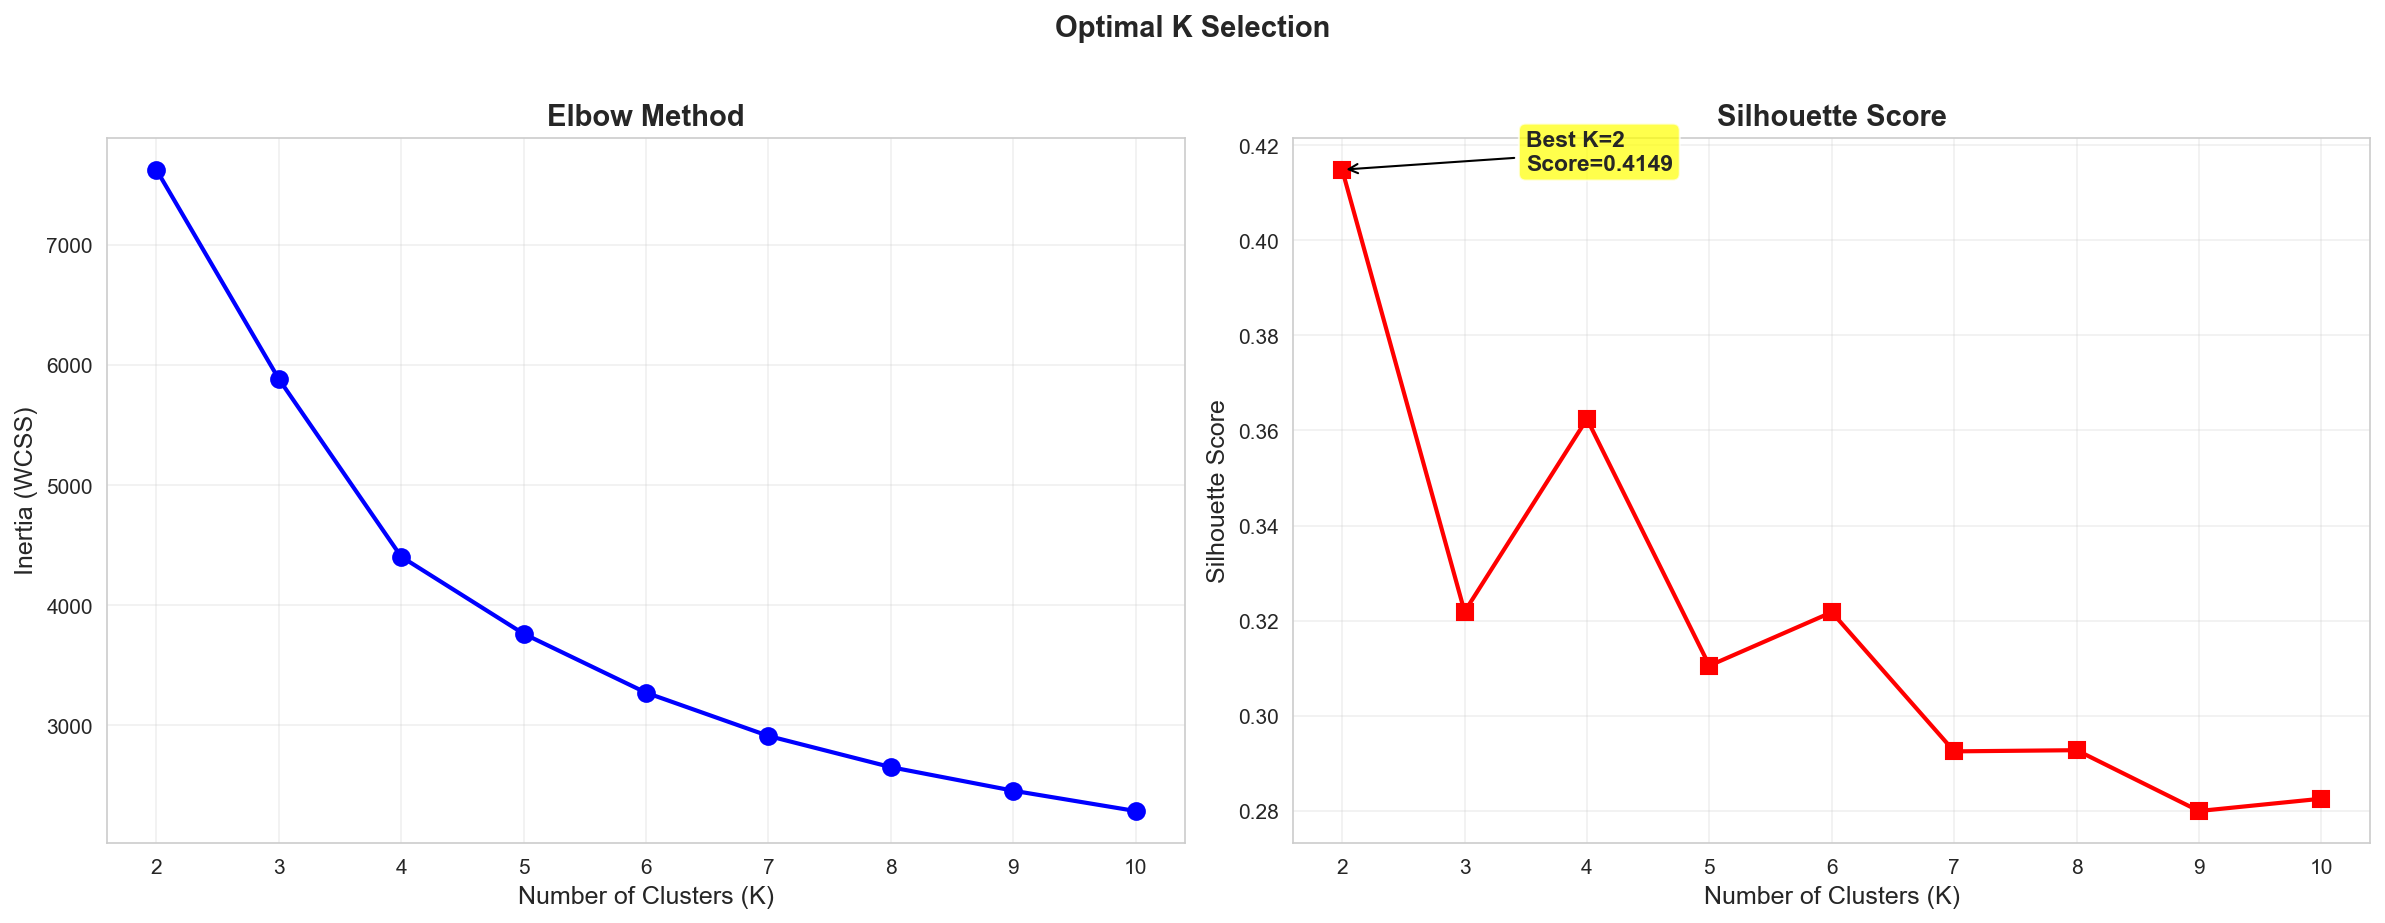
\includegraphics[width=0.85\textwidth]{figures/elbow_silhouette.png}
    \caption{Elbow method (inertia) and silhouette score curves for $K = 2\ldots10$.}
    \label{fig:elbow}
\end{figure}

\begin{figure}[H]
    \centering
    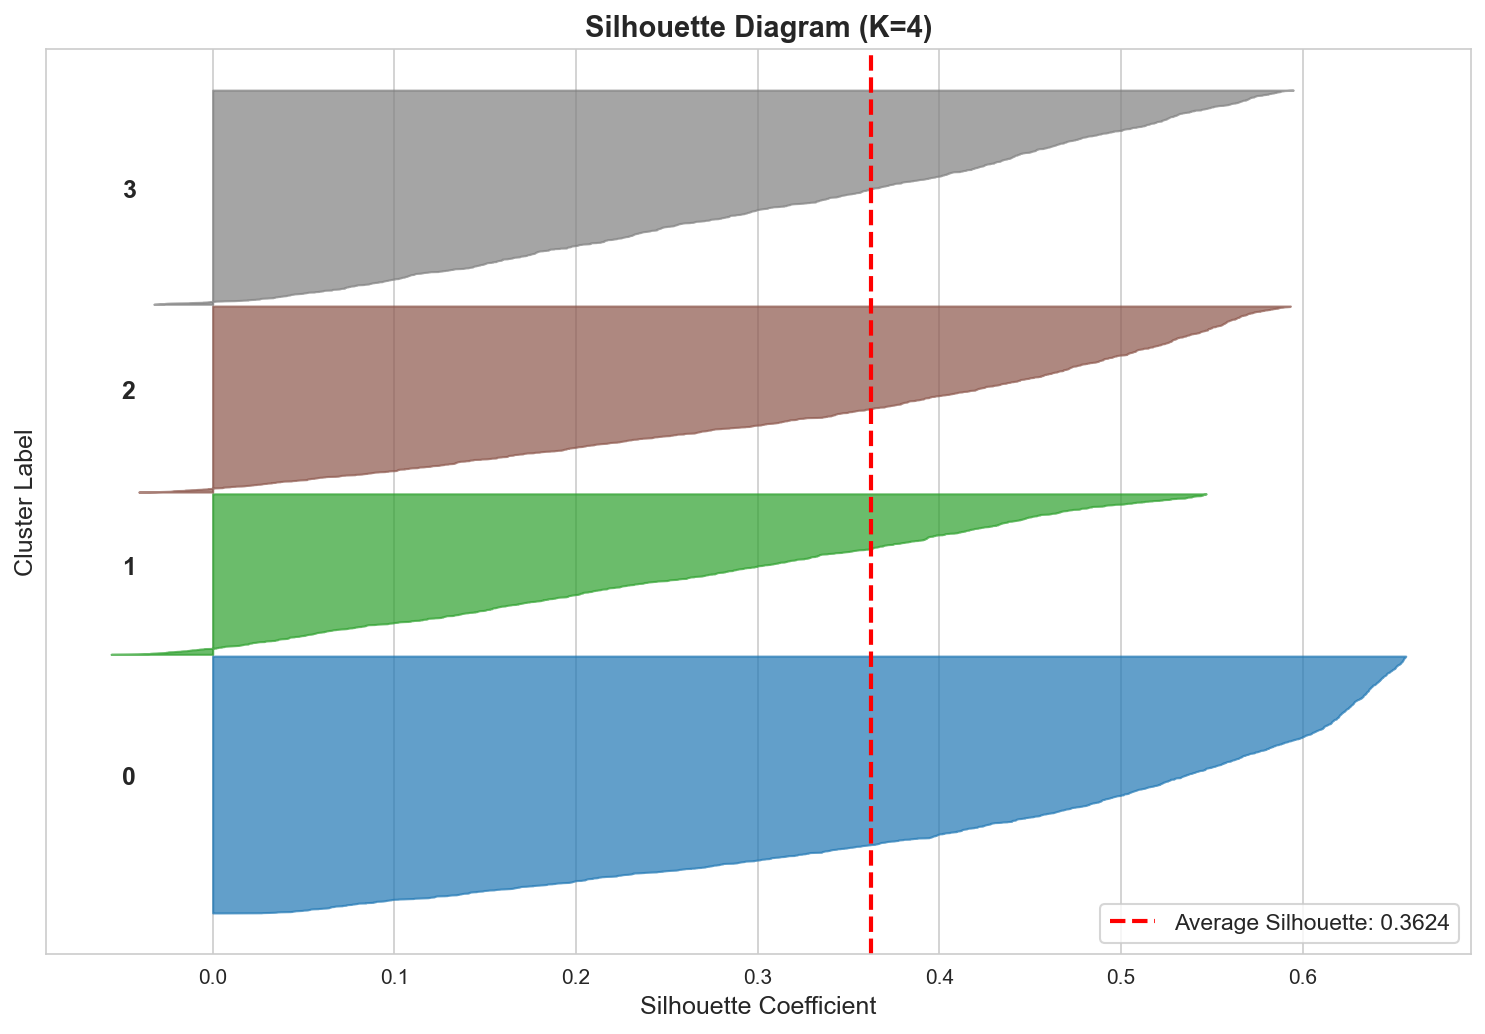
\includegraphics[width=0.85\textwidth]{figures/silhouette_diagram.png}
    \caption{Per-sample silhouette diagram for $K=4$.}
    \label{fig:silhouette_diagram}
\end{figure}

\begin{figure}[H]
    \centering
    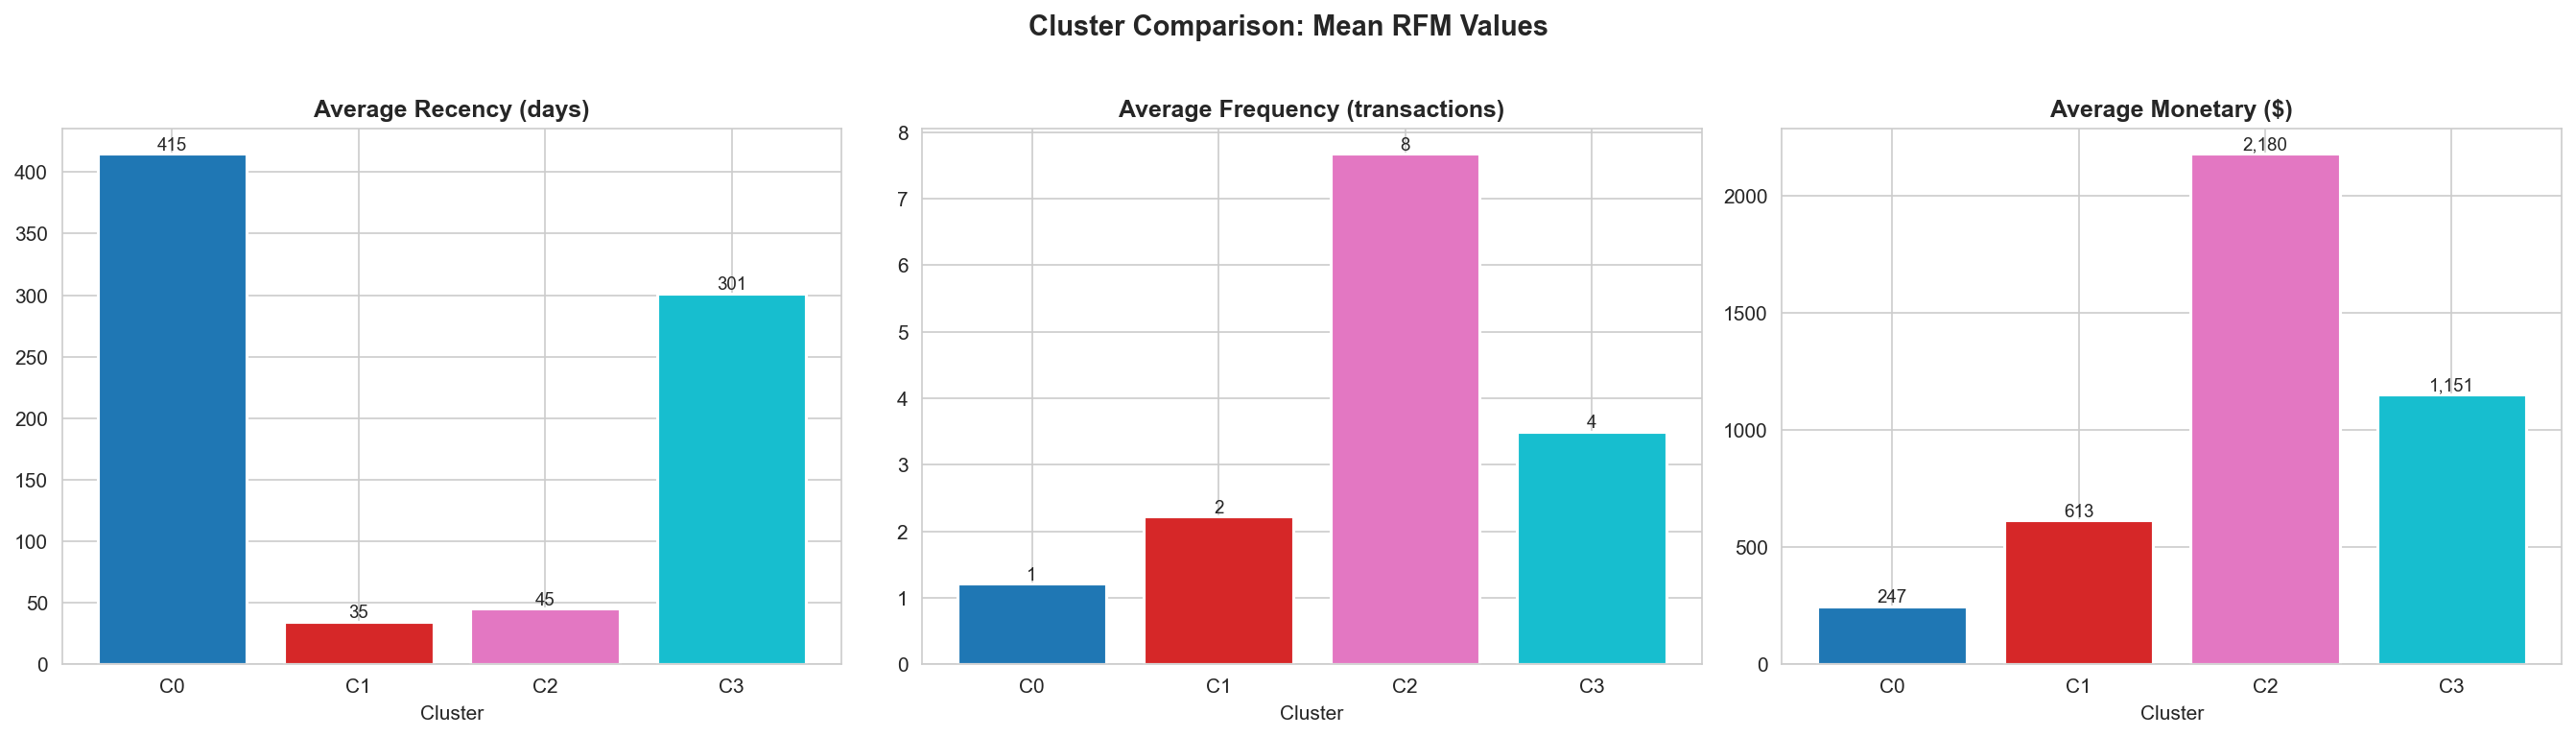
\includegraphics[width=0.85\textwidth]{figures/cluster_comparison_bars.png}
    \caption{Mean Recency, Frequency, and Monetary value per cluster.}
    \label{fig:cluster_bars}
\end{figure}

\begin{figure}[H]
    \centering
    \begin{subfigure}{0.48\textwidth}
        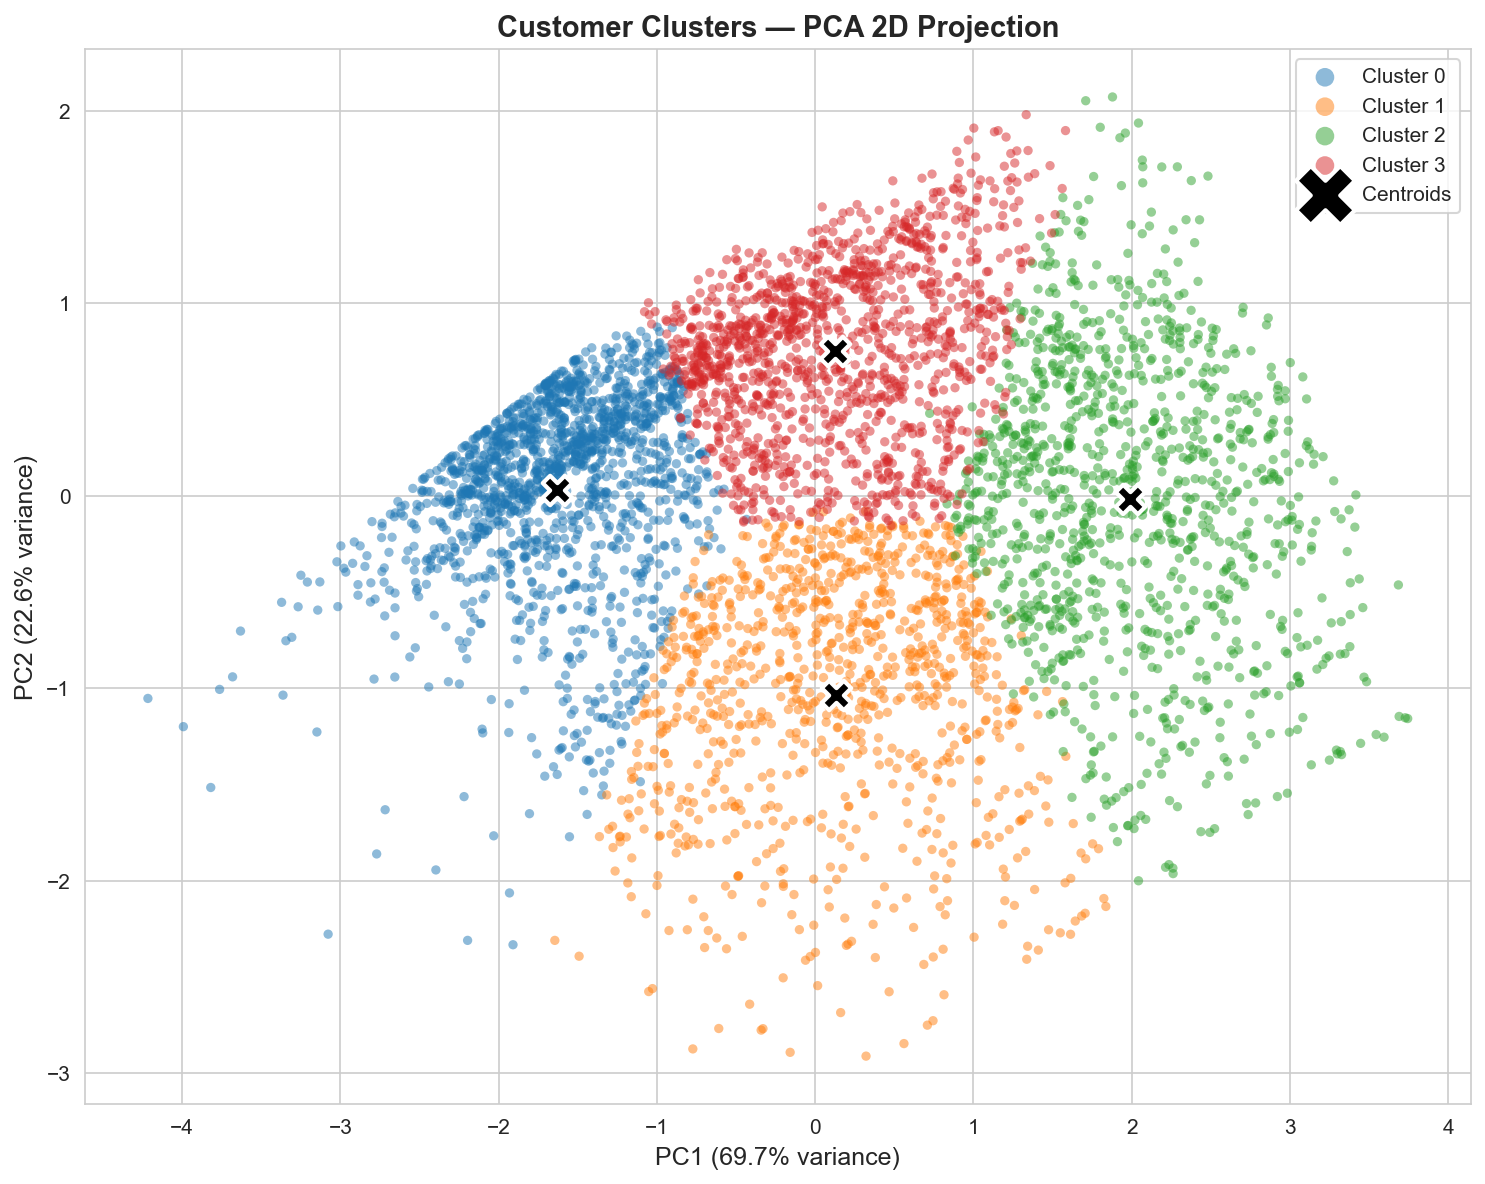
\includegraphics[width=\textwidth]{figures/clusters_pca.png}
        \caption{PCA projection.}
        \label{fig:pca}
    \end{subfigure}
    \hfill
    \begin{subfigure}{0.48\textwidth}
        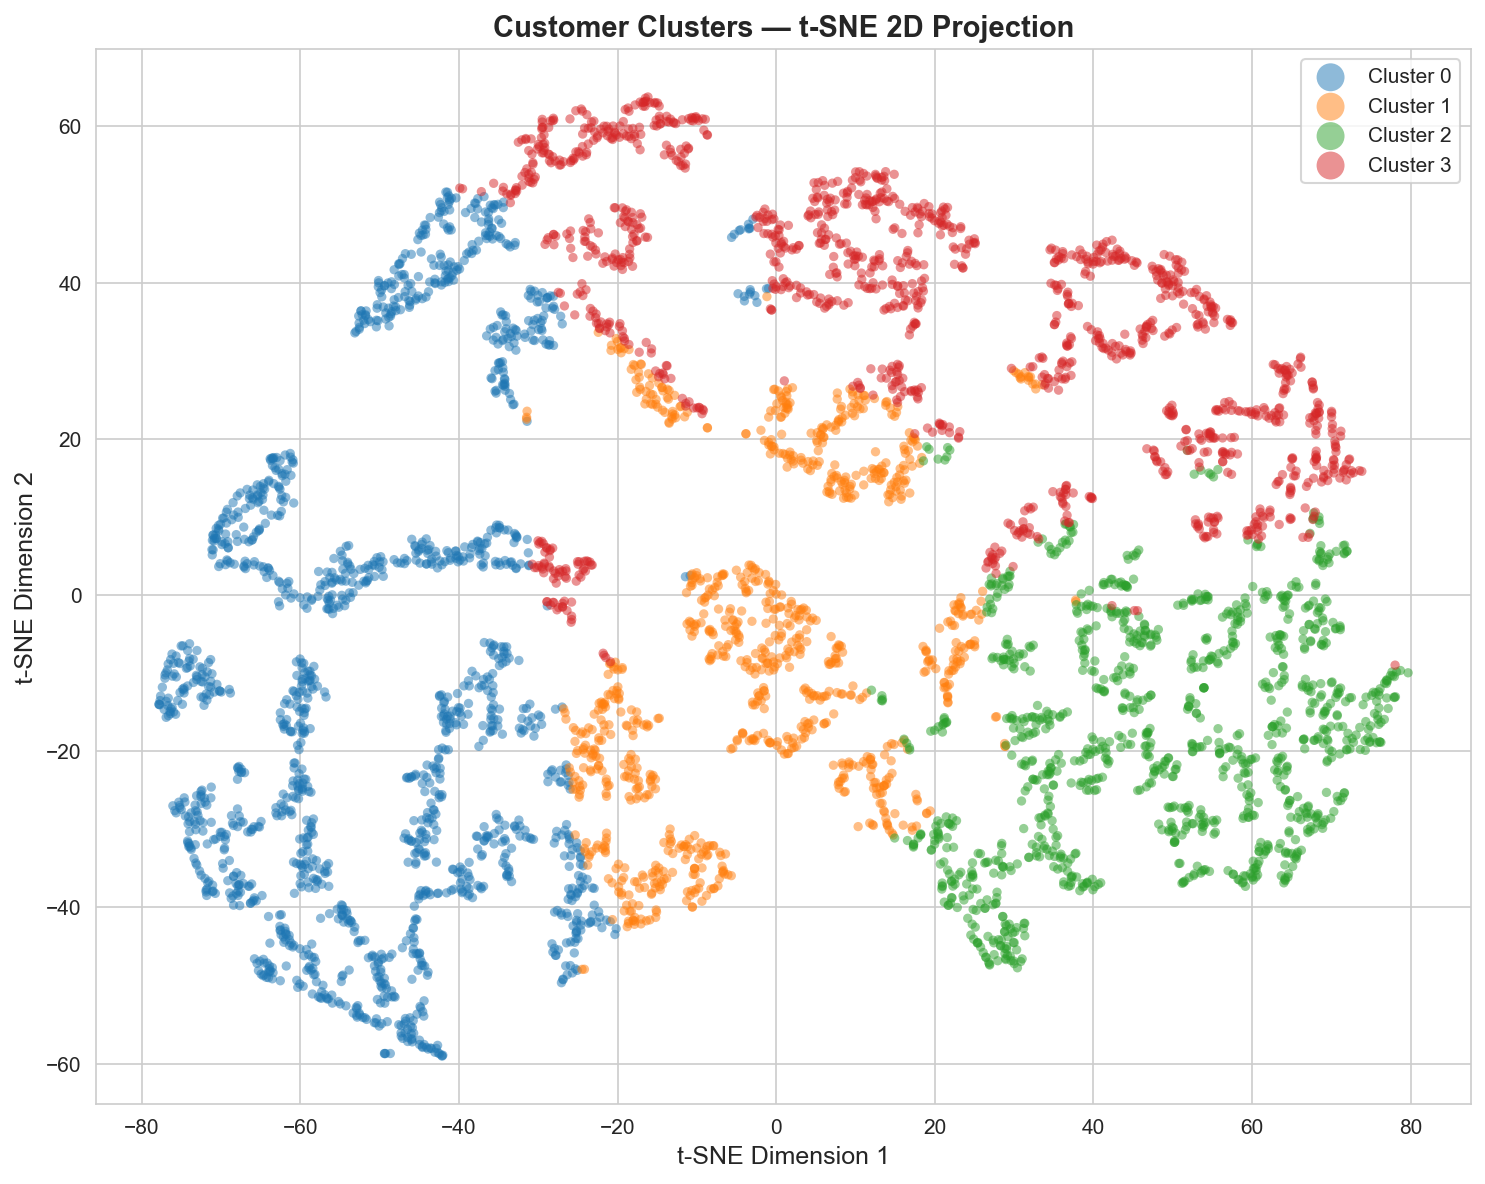
\includegraphics[width=\textwidth]{figures/clusters_tsne.png}
        \caption{t-SNE projection.}
        \label{fig:tsne}
    \end{subfigure}
    \caption{2D cluster visualisations via PCA and t-SNE.}
    \label{fig:cluster_plots}
\end{figure}

\begin{figure}[H]
    \centering
    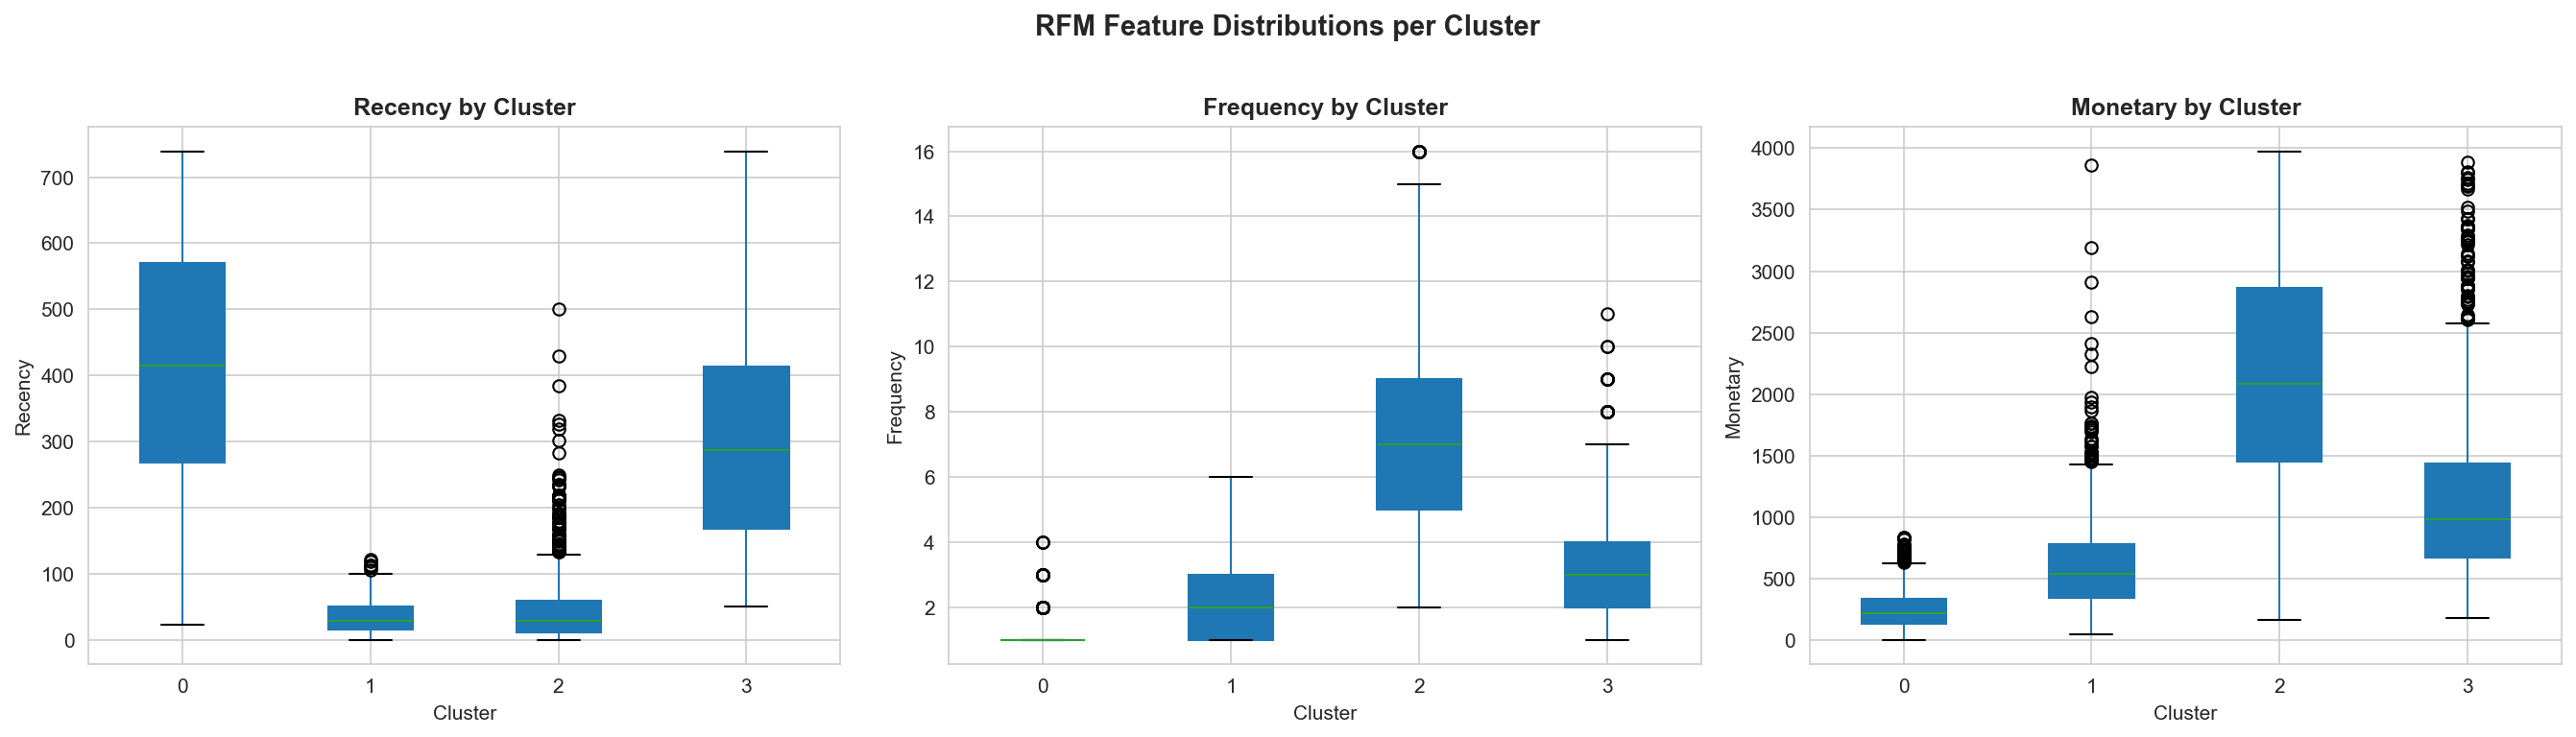
\includegraphics[width=0.85\textwidth]{figures/cluster_boxplots.png}
    \caption{RFM boxplots split by cluster, showing within-cluster spread.}
    \label{fig:cluster_boxplots}
\end{figure}

\begin{figure}[H]
    \centering
    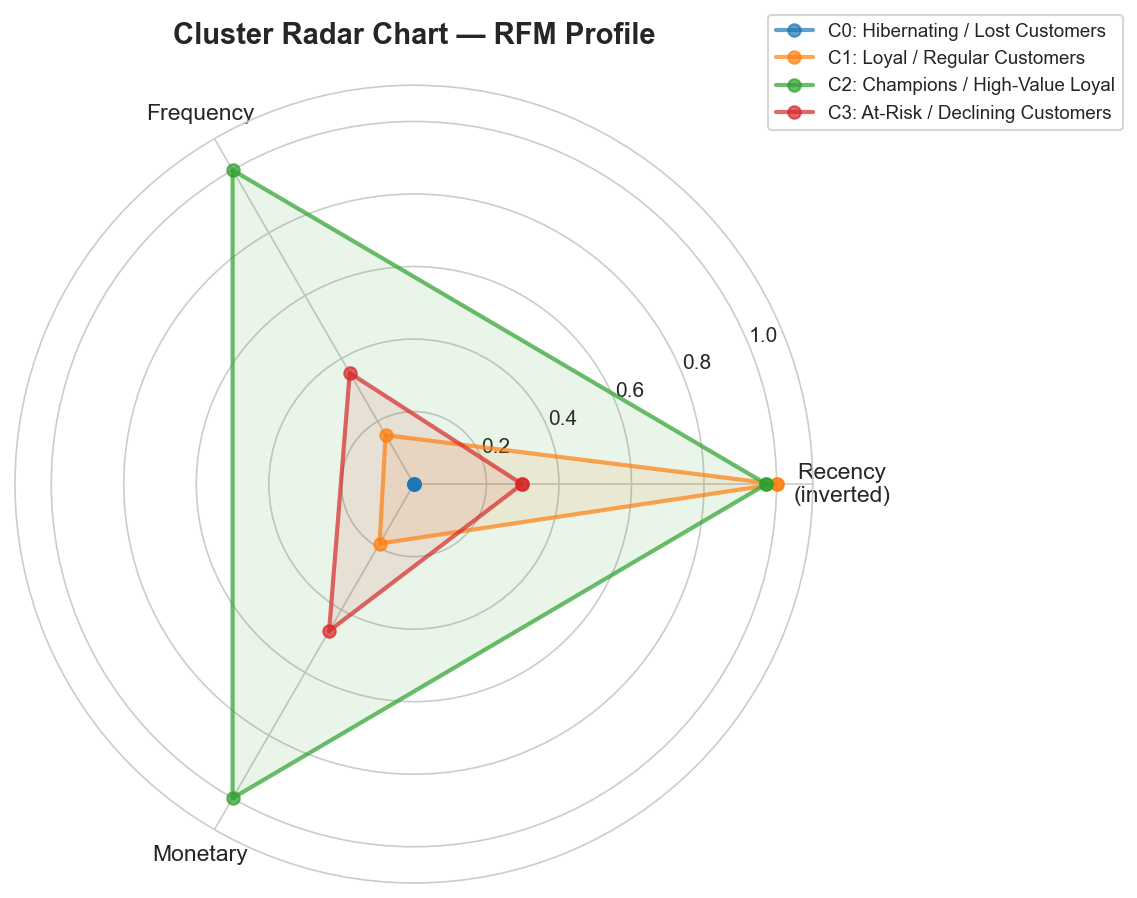
\includegraphics[width=0.7\textwidth]{figures/cluster_radar.png}
    \caption{Radar chart of normalised RFM profiles per cluster.}
    \label{fig:radar}
\end{figure}

\begin{figure}[H]
    \centering
    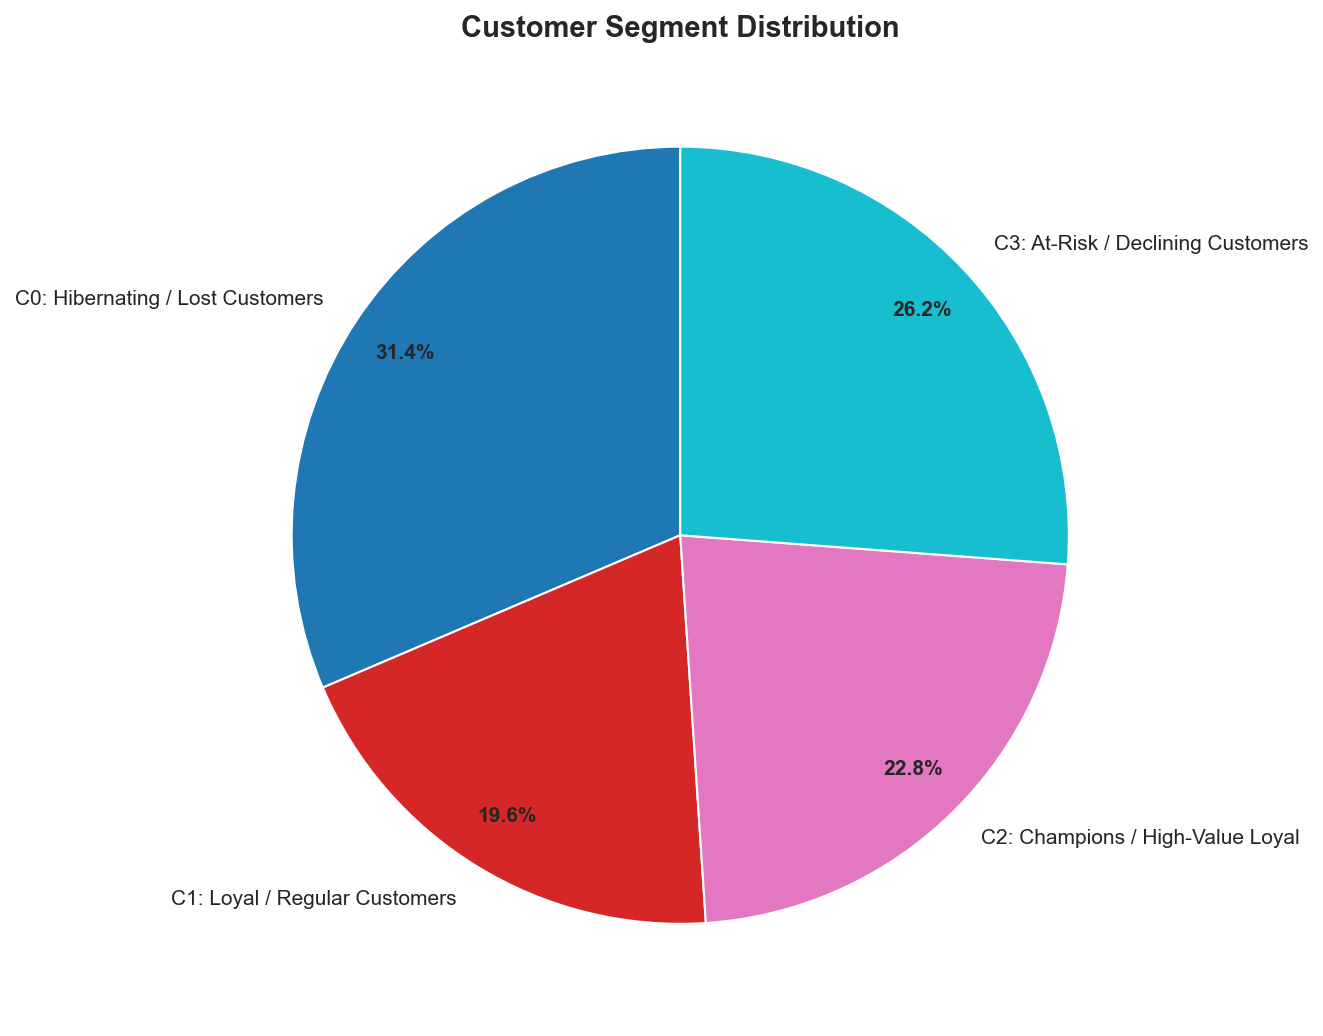
\includegraphics[width=0.7\textwidth]{figures/cluster_pie.png}
    \caption{Customer distribution across the four segments.}
    \label{fig:pie}
\end{figure}

% ============================================================
\section{Business Strategies}\label{sec:strategies}
% ============================================================

Segmentation is only as useful as the actions it generates. What follows are concrete suggestions for each cluster, based on what the RFM numbers actually say rather than generic marketing templates.

\subsection{Champions / High-Value Loyal (Cluster 2)}
\begin{itemize}[nosep]
    \item Priority access to new product launches and limited-edition ranges rewards behaviour that's already happening and gives these customers a reason to stay close.
    \item Personalised product recommendations, built from their specific purchase history, are more likely to land than anything generic.
    \item A well-structured referral scheme makes sense here; customers who buy this frequently and spend this much tend to be genuinely enthusiastic about the brand.
\end{itemize}

\subsection{Loyal / Regular Customers (Cluster 1)}
\begin{itemize}[nosep]
    \item Complementary product suggestions at checkout or in follow-up emails can raise average basket value gradually without feeling intrusive.
    \item Maintaining contact through a lightweight loyalty programme keeps the relationship active without requiring constant discounting.
    \item Occasion-based incentives, as small as a seasonal offer or a reward at a purchase milestone, can shift spending patterns over time.
\end{itemize}

\subsection{At-Risk / Declining Customers (Cluster 3)}
\begin{itemize}[nosep]
    \item A time-limited offer tied to their order history is a more targeted opening than a blanket discount; it signals that the message was written for them specifically.
    \item A short feedback form asking why their purchasing dropped off can surface service or product issues that aren't visible in transaction data alone.
    \item Price-sensitive win-back offers work for some, but the more relevant the product suggestion, the less the discount needs to do.
\end{itemize}

\subsection{Hibernating / Lost Customers (Cluster 0)}
\begin{itemize}[nosep]
    \item A re-engagement email referencing items related to their last purchase costs very little to send and will outperform a generic reactivation blast.
    \item For the subset who bought only once, the realistic goal is a second purchase, not long-term loyalty; messaging should reflect that.
    \item Customers who have not responded to multiple re-engagement attempts are probably best removed from the active mailing list to protect sender reputation.
\end{itemize}

% ============================================================
\section{Implementation}\label{sec:implementation}
% ============================================================

The codebase is written in \textbf{Python 3.13} and organised as a set of loosely coupled modules, each responsible for a distinct stage of the pipeline. This separation makes it possible to modify preprocessing logic, swap out the clustering algorithm, or adjust feature engineering without touching unrelated code. Table~\ref{tab:modules} maps each module to its function.

\begin{table}[H]
\centering
\caption{Source code modules.}
\label{tab:modules}
\begin{tabular}{@{}lp{9cm}@{}}
\toprule
\textbf{Module} & \textbf{Responsibility} \\
\midrule
\texttt{src/utils.py}          & Dataset loading, inspection, and export helpers. \\
\texttt{src/preprocessing.py}  & Full cleaning pipeline (nulls, cancellations, negatives, duplicates). \\
\texttt{src/rfm.py}            & RFM computation, log transformation, scaling, outlier removal. \\
\texttt{src/clustering.py}     & K-Means and Agglomerative training, silhouette evaluation. \\
\texttt{src/visualization.py}  & All plotting functions (distributions, elbow, PCA, t-SNE, radar). \\
\texttt{src/main.py}           & End-to-end CLI pipeline orchestrating all stages. \\
\bottomrule
\end{tabular}
\end{table}

\subsection{Reproducibility}

Full reproducibility was a deliberate design constraint. A single global constant (\texttt{RANDOM\_STATE = 42}) is passed to every stochastic operation in the pipeline, including K-Means initialisation, PCA, and t-SNE. Running the notebook top to bottom, or executing \texttt{python src/main.py} directly, will produce exactly the same cluster assignments, visualisations, and output CSVs each time.

\subsection{Dependencies}

Key libraries and tested versions:

\begin{table}[H]
\centering
\begin{tabular}{@{}ll@{}}
\toprule
\textbf{Package} & \textbf{Version} \\
\midrule
pandas       & 3.0.2  \\
numpy        & 2.4.4  \\
scikit-learn & 1.8.0  \\
matplotlib   & 3.10.8 \\
seaborn      & 0.13.2 \\
openpyxl     & $\geq$ 3.0.0 \\
scipy        & $\geq$ 1.9.0 \\
\bottomrule
\end{tabular}
\end{table}

% ============================================================
\section{Conclusion}\label{sec:conclusion}
% ============================================================

The segmentation problem at the start of this project had no obvious answer. Over a million transaction records, no pre-existing customer labels, and no prior segmentation to build from. What came out the other side were \textbf{four clusters}, each with a distinctive RFM signature that remained stable across different algorithm configurations. Tracing back through the CRISP-DM stages:

\begin{enumerate}[nosep]
    \item \textbf{Business Understanding:} the segmentation criteria were defined around commercial utility from the start; the goal was never just to produce clusters but to produce clusters that support specific decisions.
    \item \textbf{Data Understanding:} working through 1,067,371 records across 43 countries surfaced the quality issues and distributional properties that determined every subsequent choice.
    \item \textbf{Data Preparation:} preprocessing and feature transformation consumed more pipeline time than modelling, which is consistent with most real-world data projects.
    \item \textbf{Modelling:} evaluating K-Means from $K=2$ to $K=10$ systematically, rather than defaulting to a single value, gave the $K=4$ decision a quantifiable basis.
    \item \textbf{Evaluation:} running twelve experimental configurations demonstrated that the chosen setup was competitive and not simply convenient.
    \item \textbf{Deployment:} each cluster received a business label and a set of concrete recommendations rather than remaining an abstract data artefact.
\end{enumerate}

\noindent The final silhouette score of \textbf{0.3624} reflects a genuine separation between the four groups under a three-feature representation. The customer profiles produced are specific enough to drive campaign decisions and grounded in behaviour that is directly observable in the transaction records.

% ============================================================
% References
% ============================================================
\newpage
\begin{thebibliography}{9}

\bibitem{uci_retail}
Dua, D.\ and Graff, C.\ (2019).
\textit{UCI Machine Learning Repository --- Online Retail II Data Set}.
University of California, Irvine, School of Information and Computer Sciences.
\url{https://archive.ics.uci.edu/ml/datasets/Online+Retail+II}

\bibitem{rfm_theory}
Bult, J.R.\ and Wansbeek, T.\ (1995).
``Optimal Selection for Direct Mail.''
\textit{Marketing Science}, 14(4), 378--394.

\bibitem{kmeans}
Lloyd, S.P.\ (1982).
``Least squares quantization in PCM.''
\textit{IEEE Transactions on Information Theory}, 28(2), 129--137.

\bibitem{silhouette}
Rousseeuw, P.J.\ (1987).
``Silhouettes: A graphical aid to the interpretation and validation of cluster analysis.''
\textit{Journal of Computational and Applied Mathematics}, 20, 53--65.

\bibitem{crispdm}
Chapman, P.\ et al.\ (2000).
\textit{CRISP-DM 1.0: Step-by-step data mining guide}.
SPSS Inc.

\end{thebibliography}

\end{document}
